\subsection{A solvable encoder rebound family}
\label{sec:bottleneck-family}
The following family makes the mechanism explicit in a genuine bottleneck $K=1<C=2<d=3$. Its moving directions are coupled quadratic statistics, not an embedding with dormant extra coordinates.

Let $x\sim N(0,\Sigma_x)$ be one two-dimensional patch, with
\begin{equation}
 \Sigma_x=\nu_+e_+e_+^\top+\nu_-e_-e_-^\top,
 \qquad \nu_\pm\in[19/20,21/20],
\end{equation}
where $e_+,e_-$ are orthonormal. Write $q_c=\Sigma_x^{1/2}h_c$ for the filters in whitened input coordinates, and initialize
\begin{align}
 q_1&=\sqrt\epsilon\,e_++\sqrt{\epsilon/2}\,e_-,\\
 q_2&=\sqrt\epsilon\,e_+-\sqrt{\epsilon/2}\,e_-,\qquad W=(w_0,w_0).
\end{align}
Set $E_\pm=e_\pm e_\pm^\top$ and $E_\times=(e_+e_-^\top+e_-e_+^\top)/\sqrt2$. These give orthonormal coordinates for
\begin{equation}
 u=\operatorname{svec}(yy^\top-I)/\sqrt2,\qquad y=\Sigma_x^{-1/2}x.
\end{equation}
For tasks use the unit vector associated with the symmetric matrix
\begin{equation}
 \beta_{\psi,z}=\sqrt{1-z^2}(\cos\psi E_++\sin\psi E_-)+zE_\times.
\end{equation}

\begin{theorem}[Uniform encoder and projection risk gaps]
\label{thm:bottleneck-family}
Let $0<\epsilon\le1/100$, $0<w_0\le1/10$, $\eta_h>0$, and $0\le r=\eta_W/\eta_h\le10$. Use GUPA with views $x+\xi_j$, where independent $\xi_j\sim N(0,\eta\Sigma_x)$ and $0\le\eta\le1/5$. Train the actual Euclidean parameters $h,W$. Put $\theta_0=\arctan(1/2)$. For every task $Y=\beta_{\psi,z}^\top u$ with
\begin{equation}
 2\theta_0/3\le\psi\le5\theta_0/6,\qquad |z|\le1/2,
\end{equation}
the same two comparison states $t_1<t_2$ satisfy, for both optimal encoder and projection risks,
\begin{align}
 R(t_1)&\le R(0)-\Delta_1,\\
 R(t_2)&\ge R(0)+\Delta_2,
\end{align}
where
\begin{align}
 \Delta_1&=\tfrac34\sin(\theta_0/4)\sin(\theta_0/12)>0.00335,\\
 \Delta_2&=\tfrac34\sin(5\theta_0/6)\sin(\theta_0/6)>0.02181.
\end{align}
Both states are reached before $t_2<5/(76\eta_hw_0^2\epsilon)$; the loss strictly decreases and the encoder/projection ranks remain two/one. Changing $r$ in this family changes speed and energy, but not the ordered subspace path or these gaps.
\end{theorem}

\paragraph{Mechanism and exact solution.}
Equal head entries and the displayed filter symmetry persist. Put $\lambda_\pm=\norm{q_1}^2\pm q_1^\top q_2$ and $\kappa=2\Phi'(V)$ for the radial objective $L=\Phi(V)$, $V=\norm A^2$. In the increasing clock $\tau=-8\eta_h\int\kappa w^2dt$,
\begin{align}
 \lambda_\pm(\tau)&=\frac{\lambda_\pm(0)}{1-\nu_\pm\lambda_\pm(0)\tau},\\
 w^2&=w_0^2+\frac r4\sum_{j\in\{+,-\}}
             \frac{\lambda_j-\lambda_j(0)}{\nu_j}.
 \label{eq:analytic-family}
\end{align}
The encoder retains $E_\times$ and the diagonal direction $\lambda_+E_++\lambda_-E_-$; the projection retains only the latter. Its angle $\theta=\arctan(\lambda_-/\lambda_+)$ strictly decreases. The task risks are exactly
\begin{align}
 R_{\rm enc}&=(1-z^2)\sin^2(\theta-\psi),\\
 R_{\rm proj}&=z^2+(1-z^2)\sin^2(\theta-\psi).
 \label{eq:analytic-risks}
\end{align}
The two common states are $\theta_1=3\theta_0/4$ and $\theta_2=\theta_0/6$. Motion first approaches the task direction and then continues past it; the encoder itself loses readability. The fixed projection gap $z^2$ is a separate selection effect.

\begin{figure}[t]
\centering
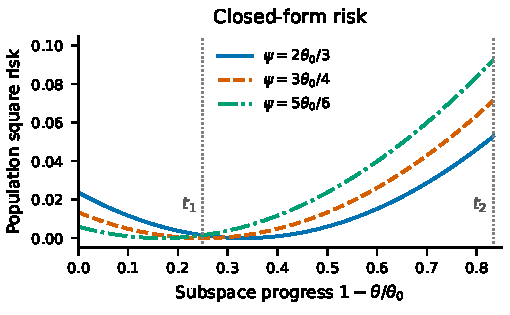
\includegraphics[width=\linewidth]{figures/analytic_bottleneck_family.pdf}
\caption{Exact risk paths in Theorem~\ref{thm:bottleneck-family}, three task directions with $z=0$. Encoder and projection risks coincide here. The same two comparison states improve and then exceed the initial risk for the entire task family. These curves evaluate the closed formula; no model is trained or numerically integrated to draw them.}
\label{fig:analytic-family}
\end{figure}

The task family contains an open cone and covers a specified $\pm5\%$ covariance range. This anisotropy range keeps covariance axes aligned with filter sums/differences and uses covariance-relative augmentation and balanced whitened initialization. Physical initial filters change with the covariance to keep that whitened balance. It is not robustness to arbitrary symmetry-breaking initialization or augmentation perturbations, nor a random-initialization probability result. The family also supplies an explicit exclusion case for rate competition: unequal rates alone do not force different directional paths. Appendix~\ref{app:task-geometry} proves the formulas, energy barrier, and reachability.
